\documentclass[12pt,a4paper]{article}
\usepackage{ctex}
\usepackage{amsmath,amscd,amsbsy,amssymb,latexsym,url,bm,amsthm}
\usepackage{epsfig,graphicx,subfigure}
\usepackage{enumitem,balance}
\usepackage{wrapfig}
\usepackage{mathrsfs,euscript}
\usepackage[usenames]{xcolor}
\usepackage{hyperref}
\usepackage[vlined,ruled,linesnumbered]{algorithm2e}
\hypersetup{colorlinks=true,linkcolor=black}

\newtheorem{theorem}{Theorem}
\newtheorem{lemma}[theorem]{Lemma}
\newtheorem{proposition}[theorem]{Proposition}
\newtheorem{corollary}[theorem]{Corollary}
\newtheorem{exercise}{Exercise}
\newtheorem*{solution}{Solution}
\newtheorem{definition}{Definition}
\theoremstyle{definition}

\renewcommand{\thefootnote}{\fnsymbol{footnote}}

\newcommand{\postscript}[2]
 {\setlength{\epsfxsize}{#2\hsize}
  \centerline{\epsfbox{#1}}}

\renewcommand{\baselinestretch}{1.0}

\setlength{\oddsidemargin}{-0.365in}
\setlength{\evensidemargin}{-0.365in}
\setlength{\topmargin}{-0.3in}
\setlength{\headheight}{0in}
\setlength{\headsep}{0in}
\setlength{\textheight}{10.1in}
\setlength{\textwidth}{7in}
\makeatletter \renewenvironment{proof}[1][Proof] {\par\pushQED{\qed}\normalfont\topsep6\p@\@plus6\p@\relax\trivlist\item[\hskip\labelsep\bfseries#1\@addpunct{.}]\ignorespaces}{\popQED\endtrivlist\@endpefalse} \makeatother
\makeatletter
\renewenvironment{solution}[1][Solution] {\par\pushQED{\qed}\normalfont\topsep6\p@\@plus6\p@\relax\trivlist\item[\hskip\labelsep\bfseries#1\@addpunct{.}]\ignorespaces}{\popQED\endtrivlist\@endpefalse} \makeatother

\begin{document}
\noindent

%========================================================================
\noindent\framebox[\linewidth]{\shortstack[c]{
\Large{\textbf{Homework 01}}\vspace{1mm}\\
CS499-Mathematical Foundations of Computer Science, Jie Li, Spring 2020.}}
\begin{center}
\footnotesize{\color{blue}Name: ������ (Hongjie Fang)  \quad Student ID: 518030910150 \quad Email: galaxies@sjtu.edu.cn}
\end{center}

\begin{enumerate}
  \item All horses are the same color; we can prove this by induction on the number of horses in a given set. Here's how: ``if there's just one horse then it's the same color as itself, so the basis is trivial. For the induction step, assume that there are $n$ horses numbered $1$ to $n$. By the induction hypothesis, horses $1$ through $(n-1)$ are the same color, and similarly horses $2$ through $n$ are the same color. But in the middle horses, $2$ through $(n-1)$, can't change color when they are in different groups; these are horses, not chameleons. So horses $1$ and $n$ must be the same color as well. Thus all $n$ horses are the same color; QED.'' What, if anything, is wrong with this reasoning?
  \begin{solution}
    During the induction step, when $n = 2$, there are no ``middle horses (horses $2$ through $(n-1)$)'' since $n - 1 = 1 < 2$, thus we can't say horse $1$ and horse $n$ (horse $2$) has the same color. As a result, we cannot draw the conclusion that every $2$ horses have the same color, so this induction proof is wrong.
  \end{solution}

  \item Find the shortest sequence of moves that transfers a tower of $n$ disks from the left peg A to the right peg B, if direct moves between $A$ and $B$ are disallowed. (Each move must be to or from the middle peg C. As usual, a larger disk must never appear above a smaller one.)
    \begin{figure}[htbp]
      \centering
      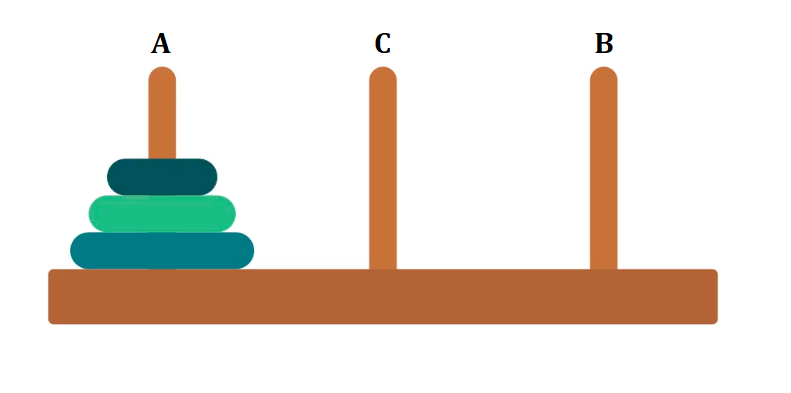
\includegraphics[width=3in]{hanoi.png}
    \end{figure}
  \begin{solution}
    Let's say $T_n$ is the minimum number of moves that will transfer $n$ disks from the left peg A to the right peg B under the given rules. Then $T_1$ is obvious $2$ ($A \rightarrow B$, $B \rightarrow C$), and we have $T_2 = 8$ ($A \rightarrow C$, $C \rightarrow B$, $A \rightarrow C$, $B \rightarrow C$, $C \rightarrow A$, $C \rightarrow B$, $A \rightarrow C$, $C \rightarrow B$).

    We have a method for transferring $n$ disks in general:
    \begin{itemize}
    \item Transfer the $(n-1)$ smallest from A to B through C (requiring $T_{n-1}$ moves);
    \item Move the largest from A to C (requiring $1$ move);
    \item Transfer the $(n-1)$ smallest from B to A through C (requiring $T_{n-1}$ moves);
    \item Move the largest from C to B (requiring $1$ move);
    \item Transfer the $(n-1)$ smallest from A to B through C (requiring $T_{n-1}$ moves).
    \end{itemize}

    With this method, we can say that
    \begin{equation}
    T_n \leq 3T_{n-1} + 2 \quad (n > 0)
    \label{eq:2.1}
    \end{equation}

    Actually this is the best way. Because at some point we have to move the largest disk from A to B, and that needs 2 steps: $A \rightarrow C$ and $C \rightarrow B$. When move the largest from A to C, we have to move the $(n-1)$ smallest from A to B through C, and this taken at least $T_{n-1}$ moves; similarly, when move the largest from C to B, we have to move the $(n-1)$ smallest from B to A through C in at least $T_{n-1}$ moves. Finally, we have to move the $(n-1)$ smallest from A to B through C in at least $T_{n-1}$ moves and finish the task. Hence,
    \begin{equation}
    T_n \geq 3T_{n-1} + 2 \quad (n > 0)
    \label{eq:2.2}
    \end{equation}

    With Equation \eqref{eq:2.1} and Equation \eqref{eq:2.2}, we have
    \begin{equation}
    T_n = 3T_{n-1} + 2 \quad (n > 0)
    \label{eq:2.3}
    \end{equation}

    With Equation \eqref{eq:2.3} and $T_0 = 1$ we can draw the conclusion that
    \begin{equation}
    T_n = 3^n - 1 \quad (n \geq 0)
    \label{eq:2.4}
    \end{equation}

    We have proved that $T_n = 3^n - 1$ is the minimum moves to transfer $n$ disks from the left peg A to the right peg B under the given rules. And the method is also given above. With the method we are able to generate the shortest path recursively.
  \end{solution}

  \item Show that, in the process of transferring a tower under the restriction of the preceding exercise, we will actually encounter every properly stacked arrangement of $n$ disks on three pegs.
  \begin{solution}
    We have proved that the shortest path takes $T_n = 3^n - 1$ moves in the solution to the preceding exercise. Let us refer to ``properly stacked arrangement of $n$ disks on three pegs'' as state. Because this is the shortest path, so every state during the transferring process must be different. There are total $3^n$ possible state, and with $T_n = 3^n - 1$ move we can go through $3^n$ different state including the initial state. So we must encounter every properly stacked arrangement of $n$ disks on three pegs when we use the method in the preceding exercise.
  \end{solution}

  \item Are there any starting and ending configurations of $n$ disks on three pegs that are more than $2^n-1$ moves apart, under Lucas's original rules?
  \begin{solution}
    No. Let $P_n$ be the total moves at most for every starting and ending configurations of $n$ disks on three pegs. We have $P_0 = 0$, $P_1 = 1$ and $P_2 = 3$ obviously. Then we consider about the largest disk.
    \begin{itemize}
        \item If the largest disk does not have to be moved, then we only need $P_{n-1}$ moves at most to get to every ending configurations under this premise.
        \item If the largest disk has to be moved, then we can:
              \begin{itemize}
                \item Transfer the other disks to the peg other than the origin peg and destination peg of the largest disk (requiring $P_{n-1}$ moves at most);
                \item Move the largest disk to the destination (requiring $1$ moves);
                \item Transfer the other disks to their destinations (requiring $P_{n-1}$ moves at most).
              \end{itemize}
              This is a workable method and it has $(2P_{n-1} + 1)$ moves at most.
    \end{itemize}

    In summary, we can finish the task in at most $(2P_{n-1} + 1)$ moves, that is,
    \begin{equation}
    P_n \leq 2P_{n-1} + 1 \quad (n \geq 3)
    \label{eq:4.1}
    \end{equation}

    With Equation \eqref{eq:4.1} and the initial state $P_0, P_1, P_2$, we can get the following formula.
    \begin{equation}
    P_n \leq 2^n - 1 \quad (n \geq 0)
    \label{eq:4.2}
    \end{equation}

    Equation \eqref{eq:4.2} shows that there are no starting and ending configurations of $n$ disks on three pegs that are more than $2^n-1$ moves apart, under Lucas's original rules.
  \end{solution}

  \item A ``Venn Diagram'' with three overlapping circles is often used to illustrate the eight possible subsets associated with three given sets. Can the sixteen possibilities that arise with four given sets be illustrated by four overlapping circles?
      \begin{figure}[h]
        \centering
        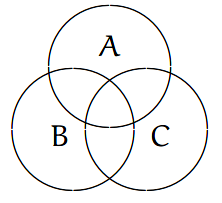
\includegraphics[width=1in]{venn.png}
      \end{figure}

  \begin{solution}
    No. Two circles can have $2$ intersection points at most. When inserting the fourth circle, we can add $6$ intersection points at most. Under the best circumstance, an intersection point means a additional region, so we can have $6$ additional regions at most, that is, totally $6+8=14$ regions at most. Thus we can not illustrate all 16 possibilities that arise with four given sets by four overlapping circles.
  \end{solution}

  \item Some of the regions defined by $n$ lines in the plane are infinite, while others are bounded. What's the maximum possible number of bounded regions?
  \begin{solution}
    Let's say $R_n$ is the maximum possible number of bounded regions when there are $n$ line(s), then obvious $R_1 = R_2 = 0$ and $R_3 = 1$, since at least three lines can form a bounded region. Consider a new line $l$, which can have at most $(n-1)$ intersection points with the previous $(n-1)$ lines. As a result, the new line $l$ can form at most $(n-2)$ additional regions. So we have:
    \begin{equation}
        R_n \leq R_{n-1} + (n-2)  \quad (n \geq 4)
        \label{eq:6.1}
    \end{equation}

    Actually, we can achieve the equality in Equation \eqref{eq:6.1}, so we have the following formula.
    \begin{equation}
        R_n = R_{n-1} + (n-2) \quad (n \geq 4)
        \label{eq:6.2}
    \end{equation}

    With Equation \eqref{eq:6.2} we can get the following general formula of $R_n$ simply by induction.
    \begin{equation}
        R_n = \frac{1}{2} (n-1)(n-2) (n \geq 1)
        \label{eq:6.3}
    \end{equation}

    In conclusion, we can get the maximum possible number of $R_n = \frac{1}{2} (n-1)(n-2)$ bounded regions with $n (n \geq 1)$ line(s).
  \end{solution}

  \item Let $H(n)=J(n+1)-J(n)$. Equation (1.8) in the textbook tells us that $H(2n)=2$, and $H(2n+1) = J(2n+2)-J(2n+1)=(2J(n+1) - 1) - (2J(n)+1) = 2H(n) - 2$, for all $n \ge 1$. Therefore it seems possible to prove that $H(n)=2$ for all $n$ by induction on $n$. What's wrong here?
  \begin{solution}
    $H(1) = J(2) - J(1) = (2J(1) - 1) - J(1) = 0 \ne 2$, so the basis step of the induction is wrong. As a result, we can not get $H(n) = 2$ for all $n$.
  \end{solution}
\end{enumerate}
%========================================================================
\end{document}
